\section{Permission and role management}

Unplagged does offer an extensive permission and role management, which controls access to pages and entities within the system. It contains two important parts: roles and permissions. A permission is a actually a single right on a resource within the portal and roles are collections of permissions.

\subsection{Roles}

Roles are being used for assigning pre-defined sets of permissions to a single user in different situations. There exist 4 different types of roles, with different characteristics:

\begin{itemize}
\item    	Global roles
\item   	User roles  
\item    	Case default roles
\item   	Case roles
\end{itemize}

Besides the different role types, there exists a concept of role inheritance in our system. One role can inherit from another one, in this case, a user does have the joined rights of the main role and the inherited role as well. 

\textbf{Global roles}

To make this more visual, let's start with the global roles. Global roles include default roles for guests, registered users and admins. A non-registered user does have the guest role by default, a registered user the user role. Since administrative users need some more privilleges, they need the admin role as well. Since the admin role is an inheritable role, it extends the user role and user get's all the rights which are either in the user role or in the admin role.

\textbf{User roles}

When a user registeres on the plattform, a copy of the global user role is created and assigned to the user as it's default role. This role can be modified for each user without influencing other users, so one user can have completely different rights than another one.

\textbf{Case default roles}

All the permissions defined in the roles described above are related to all cases the user is taking part in. Although often it is necessary to add different rights to a user in different cases. For example in one case a user can access all documents, in another one the user can access the files area only. For this case two case default roles are provided: an admin role and a collaborator role, they can be seen as a global role on the case level, used as templates for all cases. 

\textbf{Case roles}

When a new case is created, the same process as described for the user roles takes part, a copy of the case default roles is created, they can be assigned to any collaborator of the case (figure \ref{fig:collaborators-form}). A case role can be added to a user by accessing the Case > Edit form in the 'case collaborators' section. An autocompletion field let's the user search for collaborators by username and then through a dropdown, the role can be selected, as shown in figure \ref{fig:collaborators-form}.

\begin{figure}[!h]
  \centering
  \fbox{
    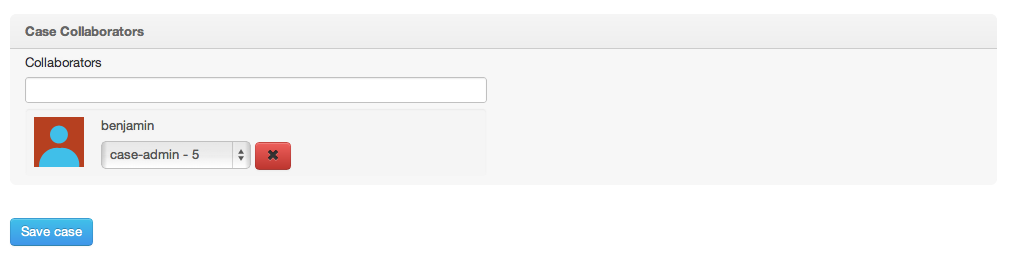
\includegraphics[width=0.97\textwidth]{images/collaborators-form.png}
  }
  \caption{Roles overview}
  \label{fig:collaborators-form}
\end{figure}

All the different roles used in Unplagged can be managed in the Administration > Roles area (figure \ref{fig:roles-list} and figure \ref{fig:roles-form}).

\begin{figure}[!h]
  \centering
  \fbox{
    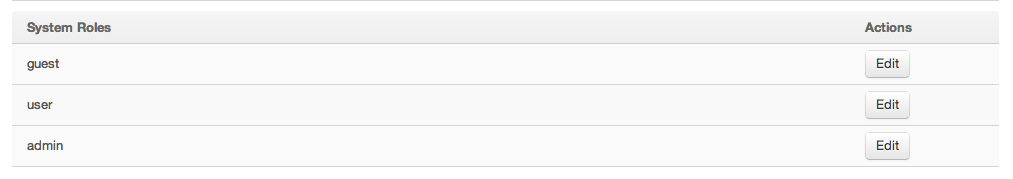
\includegraphics[width=0.97\textwidth]{images/roles-list.png}
  }
  \caption{Roles overview}
  \label{fig:roles-list}
\end{figure}

\begin{figure}[!h]
  \centering
  \fbox{
    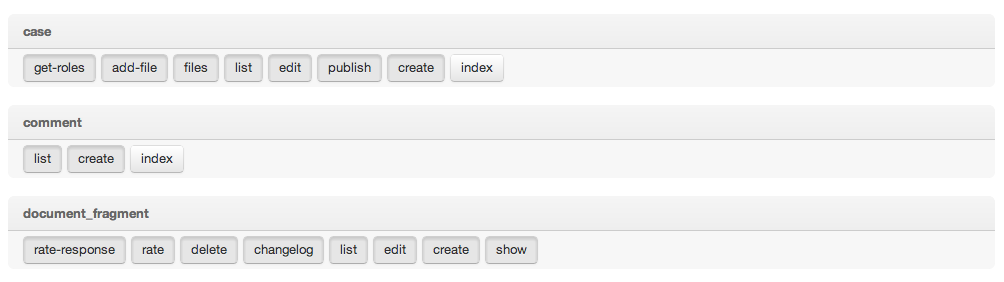
\includegraphics[width=0.97\textwidth]{images/roles-form.png}
  }
  \caption{Role form}
  \label{fig:roles-form}
\end{figure}

\subsection{Permission types}

There exist two permission types which are extending from an abstract permission model – page permissions and model permissions. How they differ from each other will be described further on. Usually a permission is related to a specific object, but we also do have global permissions, which define access to all entities of a kind. 

A single permission basically contains four properties:

\begin{itemize}
\item      type – what model / page type is protected (e.g. document, file, case) 
\item      action – what action of the type (e.g. read, list, create)
\item      base – which entity is protected (e.g. a real entity id or a * for global rights)
\item      permission type – page permission or model permission
\end{itemize}

When a user does not have access to a page resource or a model resource, one is redirected to the previously accessed page automatically.

\textbf{Model permissions}

The ModelPermission entity manages access to single objects within the system, this includes for example cases, files, documents, fragments and comments. Each of them currently has a fixed set of permission actions, based on the CRUD design pattern – create, read, update, delete and a fifth one called authorize. The authorize permission allows a user to control the permissions on a specific entity.

If the user does have the authorize permission on an entity, the form to edit them, can accessed through the actions menu in the list view of the object, as shown in figure \ref{fig:add-model-permission}. 

\begin{figure}[!h]
  \centering
  \fbox{
    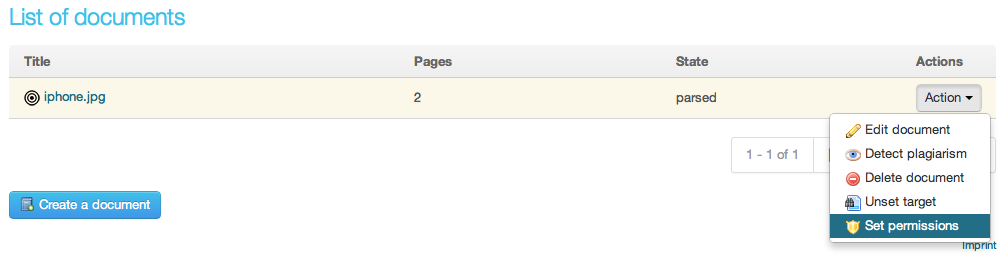
\includegraphics[width=0.97\textwidth]{images/add-model-permission.png}
  }
  \caption{Access form for editing model permissions}
  \label{fig:add-model-permission}
\end{figure}

The form provided to set the permissions offers an autocompletion textfield at the top, where usernames can be searched and afterwards the permissions can be defined by enabling or disabling the buttons below the username (figure \ref{fig:set-model-permissions}).

\begin{figure}[!h]
  \centering
  \fbox{
    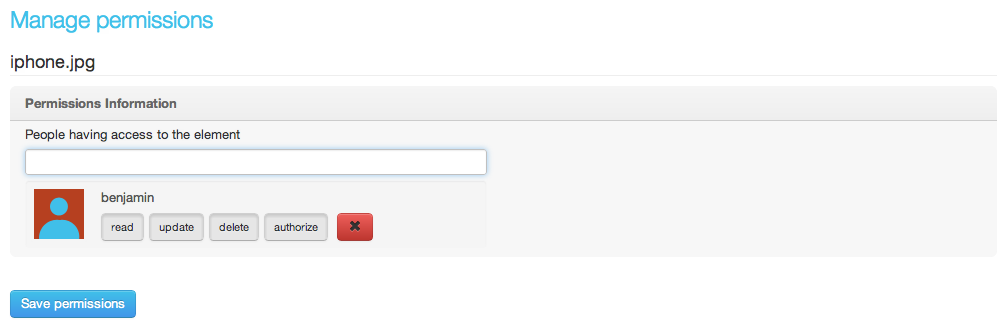
\includegraphics[width=0.97\textwidth]{images/set-model-permissions.png}
  }
  \caption{Set permissions on an entity}
  \label{fig:set-model-permissions}
\end{figure}

The permission check on models does have to be done by hand in any controller action, where needed. A simple selection of the required permission and then a call of the hasPermission-method on the user role is sufficient. The following example checks the users read permission on a specific document:

\begin{lstlisting}[caption=Checking the user permission on an entity]
$permission = $this->_em->getRepository('Application_Model_ModelPermission')->findOneBy(array('type'=>'document', 'action'=>'read', 'base'=>$document));
if(Zend_Registry::getInstance()->user->getRole()->hasPermission($permission)){
	// user has access
}
\end{lstlisting}

\textbf{Page permissions}

The second type of permissions are the page permissions. They control access to controller and action methods. This means, they define whether a user can for example access the page /document/list or not. The available permissions are being generated on each deployment of the site automatically. So when a new action in a controller is created, it will be available as a new permission after the next deployment.
